\documentclass[12pt]{article}

\usepackage{amsmath}
\usepackage{amssymb}
\usepackage{enumitem}
\usepackage[margin=1in]{geometry}

\usepackage{tikz}
\usetikzlibrary{arrows.meta,decorations.pathmorphing,calc,angles,quotes}

\setlist[enumerate,1]{label=\arabic*.}

\begin{document}

\begin{center}
\Large \textbf{ULTRA-HARD PHYSICS PAPER}
\end{center}

\begin{enumerate}

\item \textbf{Wedge–Spring Coupled Dynamics}


A wedge of mass $M$ rests on a perfectly smooth horizontal surface and has an incline making angle $\theta$ with the horizontal. A small block of mass $m$ is attached to a light spring of stiffness $k$, whose other end is fixed at the top of the incline. The spring lies along the incline and is initially compressed by a distance $x$. The block is released from rest relative to the wedge. Neglect any rotational effects of the wedge and assume motion remains planar.

During the subsequent motion, determine the maximum horizontal velocity attained by the wedge before the spring reaches its natural length for the first time.

\begin{center}
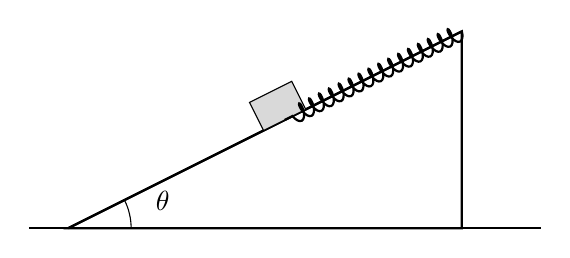
\begin{tikzpicture}[scale=1]

% Parameters
\def\base{5}
\def\height{2.5}

% Ground
\draw[thick] (-0.5,0) -- (6,0);

% Wedge (proper triangle)
\draw[thick] (0,0) -- (\base,0) -- (\base,\height) -- cycle;

% Incline
\draw[thick] (0,0) -- (\base,\height);

% Compute angle of incline
\pgfmathsetmacro{\angle}{atan(\height/\base)}

% Block position along incline
\coordinate (A) at ($(0,0)!0.55!(\base,\height)$);

% Block (rotated along incline)
\begin{scope}[shift={(A)}, rotate=\angle]
\draw[fill=gray!30] (-0.3,0) rectangle (0.3,0.4);
\end{scope}

% Spring from top of incline to block
\draw[
thick,
decorate,
decoration={coil,aspect=0.4,segment length=4pt,amplitude=3pt}
] (\base,\height) -- (A);

% Angle theta at base
\draw (0.8,0) arc (0:\angle:0.8);
\node at (1.2,0.35) {$\theta$};

\end{tikzpicture}
\end{center}

A) $\dfrac{m}{M+m}\sqrt{\dfrac{kx^2}{m}}$

B) $\dfrac{m}{M+m}\sqrt{\dfrac{2kx^2}{m}}$

C) $\dfrac{m\cos\theta}{M+m}\sqrt{\dfrac{2kx^2}{m}}$

D) $\dfrac{m}{M}\sqrt{\dfrac{2kx^2}{m}}$

\item \textbf{Velocity Selector Perturbation Theory}

A charged particle of charge $q$ and mass $m$ enters a region containing mutually perpendicular uniform electric field $E$ and magnetic field $B$. The particle’s initial velocity is $v = v_0 + \Delta v$, where $v_0 = E/B$ and $\Delta v \ll v_0$. The particle undergoes a trochoidal trajectory due to imperfect velocity selection.

To first order in $\Delta v$, determine the radius of curvature of the instantaneous circular component of motion.

A) $\dfrac{m\Delta v}{qB}$

B) $\dfrac{m(v_0+\Delta v)}{qB}$

C) $\dfrac{mE}{qB^2}$

D) $\dfrac{mv_0}{qB}$

\item \textbf{Electromagnetic Damping of Rotating Rod} \\ 


A uniform conducting rod of length $L$, resistance $R$, and mass $m$ is hinged at one end and released from rest from the horizontal position. A uniform magnetic field $B$ is directed perpendicular to the plane of motion. As the rod swings downward, motional emf induces current causing energy dissipation.

Assuming the energy loss due to induced current remains small compared to gravitational potential change, determine the angular velocity of the rod at the lowest point to first order in magnetic damping.

\begin{center}
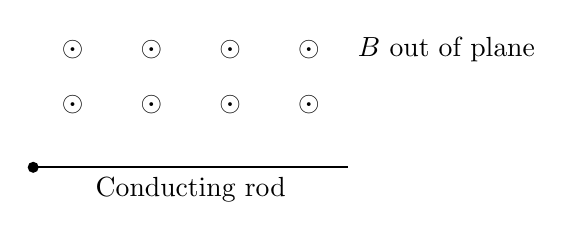
\begin{tikzpicture}[scale=1]

% Pivot
\fill (0,0) circle (2pt);

% Rod
\draw[thick] (0,0) -- (4,0);

% Label
\node[below] at (2,0) {Conducting rod};

% Magnetic field dots
\foreach \x in {0.5,1.5,2.5,3.5}
{
\foreach \y in {0.8,1.5}
{
\node at (\x,\y) {$\odot$};
}
}

\node[right] at (4,1.5) {$B$ out of plane};

\end{tikzpicture}
\end{center}

A) $\sqrt{\dfrac{3g}{L}}$

B) $\sqrt{\dfrac{3g}{L}-\dfrac{3B^2L^2}{2mR}}$

C) $\sqrt{\dfrac{6g}{L}}$

D) $\sqrt{\dfrac{3g}{L}-\dfrac{B^2L^2}{mR}}$

\item \textbf{Nonlinear Equation of State Work Calculation}

An ideal gas is taken through a reversible quasi-static process obeying the equation  
\[
P = aV + \frac{b}{V},
\]
where $a$ and $b$ are positive constants. The gas expands slowly from volume $V_1$ to $V_2$ while maintaining thermal equilibrium internally. Assume no phase transitions occur.

Calculate the total work done by the gas during the expansion.

A) $\dfrac{a}{2}(V_2^2-V_1^2)+b\ln\dfrac{V_2}{V_1}$

B) $a(V_2-V_1)+\dfrac{b}{V_2-V_1}$

C) $\dfrac{a}{2}(V_2-V_1)^2+b\ln\dfrac{V_2}{V_1}$

D) $aV_2^2+b\ln V_2$

\item \textbf{Radial Oscillations in Central Potential}

A satellite of negligible size moves in a circular orbit of radius $R$ around a planet under inverse-square gravitational attraction. The orbit is slightly perturbed radially by a small displacement $\delta R$ without changing angular momentum significantly.

Determine the frequency of small radial oscillations (epicyclic frequency) in comparison to the orbital angular frequency.

A) Equal to orbital frequency  

B) Twice orbital frequency  

C) Half orbital frequency  

D) Zero  

\item \textbf{Small Oscillations in Polynomial Potential}

A particle of mass $m$ moves along the x-axis under a conservative force derived from potential  
\[
U(x) = \alpha x^6 - \beta x^4,
\]
where $\alpha, \beta > 0$. The particle is slightly displaced about a stable equilibrium position and executes small oscillations.

Determine how the angular frequency of oscillation depends parametrically on $\alpha$ and $\beta$.

A) Proportional to $\sqrt{\beta}$

B) Proportional to $\beta$

C) Proportional to $\sqrt{\alpha}$

D) Proportional to $\sqrt{\dfrac{\beta^2}{\alpha}}$

\item \textbf{Impulse Driven Coupled Oscillator}

Two identical blocks each of mass $m$ are connected by a light spring of constant $k$ on a frictionless surface. A constant force $F$ acts on one block for a short duration $t$, after which it is suddenly removed. Assume $t$ is much smaller than the natural period of oscillation.

Determine the maximum compression of the spring during subsequent motion.

A) $\dfrac{F^2t^2}{8mk}$

B) $\dfrac{F^2t^2}{4mk}$

C) $\dfrac{F^2t^2}{2mk}$

D) $\dfrac{F^2t^2}{mk}$

\item \textbf{Rotating Loop in Magnetic Field} \\ 


A circular conducting loop of radius $R$ rotates with constant angular velocity $\omega$ about a diameter while placed in a uniform magnetic field $B$. The axis of rotation lies in the plane of the loop and is perpendicular to the magnetic field direction.

Determine the average induced emf over one complete rotation.

\begin{center}
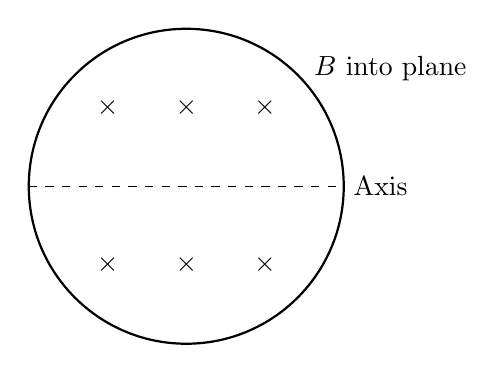
\begin{tikzpicture}[scale=1]

% Loop
\draw[thick] (0,0) circle (2);

% Axis (diameter)
\draw[dashed] (-2,0) -- (2,0);
\node[right] at (2,0) {Axis};

% Magnetic field crosses
\foreach \x in {-1,0,1}
{
\foreach \y in {-1,1}
{
\node at (\x,\y) {$\times$};
}
}

\node[right] at (1.5,1.5) {$B$ into plane};

\end{tikzpicture}
\end{center}

A) $0$

B) $\dfrac{B\omega R^2}{2}$

C) $B\omega R^2$

D) $\dfrac{B\omega R}{2}$

\item \textbf{Variable Gravity Projectile Motion}

A projectile is launched vertically upward with speed $u$ from the surface of a planet where gravitational acceleration decreases linearly with height according to  
\[
g(h) = g_0\left(1 - \frac{h}{R}\right).
\]
Assume $h \ll R$ but retain the first correction term.

Determine the approximate maximum height reached.

A) $\dfrac{u^2}{2g_0}$

B) $\dfrac{u^2}{2g_0}\left(1+\dfrac{u^2}{3g_0R}\right)$

C) $\dfrac{u^2}{2g_0}\left(1-\dfrac{u^2}{3g_0R}\right)$

D) $\dfrac{u^2}{2g_0R}$

\item \textbf{Capacitor Plate Separation Dynamics}

A parallel-plate capacitor with plate area $A$ is connected to an ideal battery maintaining constant voltage $V$. The plate separation is increased slowly from $d$ to $2d$ while neglecting fringing effects and edge fields.

Determine how the electrostatic force between plates varies with separation during the process.

A) Proportional to $1/d^2$

B) Proportional to $1/d$

C) Constant

D) Proportional to $d$

\item \textbf{Bohr Model Angular Momentum Scaling}

In the Bohr model of hydrogen atom, the electron transitions between stationary states such that its angular momentum increases by a factor of 3. Assume no relativistic corrections and neglect spin effects.

Determine the factor by which the total energy of the electron changes.

A) $9E$

B) $\dfrac{E}{9}$

C) $3E$

D) $\dfrac{E}{3}$

\item \textbf{Underdamped Oscillator Peak Separation}

A linear damped harmonic oscillator has natural angular frequency $\omega_0$ and damping ratio $\zeta < 1$. The system is displaced and released from rest.

Determine the time interval between successive displacement maxima.

A) $\dfrac{2\pi}{\omega_0}$

B) $\dfrac{2\pi}{\omega_0\sqrt{1-\zeta^2}}$

C) $\dfrac{\pi}{\omega_0}$

D) $\dfrac{1}{\zeta\omega_0}$

\item \textbf{Fringe Visibility with Unequal Intensities}

In Young’s double slit experiment, the intensity of light emerging from slit 1 is twice that from slit 2. Assume coherent monochromatic light and negligible slit width.

Determine the fringe visibility of the resulting interference pattern.

A) $\dfrac{2\sqrt{2}}{3}$

B) $\dfrac{1}{2}$

C) $1$

D) $\dfrac{2}{3}$

\item \textbf{Loop-the-Loop Energy Constraint} \\ 


A small block slides without friction along a vertical circular track of radius $R$. It is released from rest from a height $h$ above the lowest point. Air resistance is negligible and the track is rigid.

Determine the minimum height required so that the block just maintains contact at the top of the loop.

\begin{center}
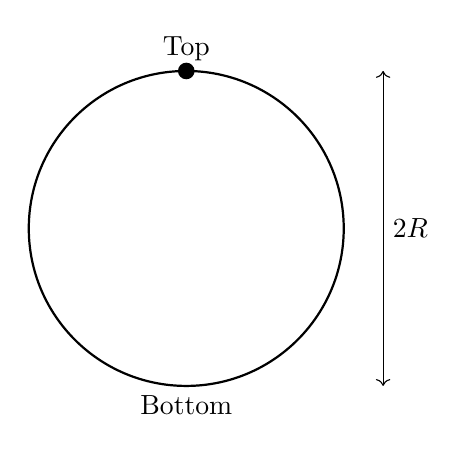
\begin{tikzpicture}[scale=1]

% Loop
\draw[thick] (0,0) circle (2);

% Block at top
\fill (0,2) circle (3pt);
\node[above] at (0,2) {Top};

% Bottom
\node[below] at (0,-2) {Bottom};

% Height arrow
\draw[<->] (2.5,-2) -- (2.5,2);
\node[right] at (2.5,0) {$2R$};

\end{tikzpicture}
\end{center}

A) $\dfrac{5R}{2}$

B) $2R$

C) $\dfrac{3R}{2}$

D) $3R$

\item \textbf{Magnetic Interaction Between Loop and Wire} \\ 


A circular conducting loop carrying steady current $I$ lies in the same plane as a long straight wire carrying equal current. The loop is positioned such that the wire is tangent to the loop. Consider magnetic forces on all current elements.

Determine the net torque acting on the loop about its center.

\begin{center}
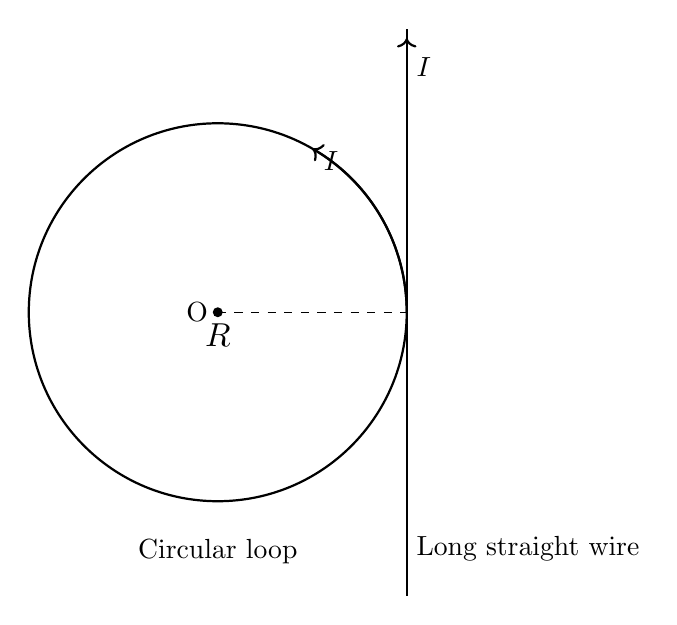
\begin{tikzpicture}[scale=1.2]

% Circle (loop)
\draw[thick] (0,0) circle (2);

% Current direction in loop
\draw[->,thick] (2,0) arc (0:60:2);
\node at (1.2,1.6) {$I$};

% Straight wire tangent to circle
\draw[thick] (2,-3) -- (2,3);

% Current in straight wire
\draw[->,thick] (2,2.2) -- (2,2.9);
\node[right] at (2,2.6) {$I$};

% Center point
\fill (0,0) circle (1.5pt);
\node[left] at (0,0) {O};

% Radius line
\draw[dashed] (0,0) -- (2,0);
\node[midway,below] {$R$};

% Label wire
\node[right] at (2,-2.5) {Long straight wire};

% Label loop
\node[below] at (0,-2.3) {Circular loop};

\end{tikzpicture}
\end{center}

A) Zero  

B) Non-zero  

C) Depends on current direction  

D) Depends on radius  

\end{enumerate}

\end{document}